% Original book diagram: fig:robotic_digital_twin_workflow_intro
% Book source: sections/front/introduction.tex
% Original diagram authorship retained. Visual design: Ziad Mosalam.
\documentclass[11pt,border=8pt]{standalone}
\usepackage{amsmath,amssymb,graphicx,tikz}
\usetikzlibrary{arrows.meta,automata,positioning,calc,shapes.geometric,fit,backgrounds,patterns}
\newcommand{\vect}[1]{\mathbf{#1}}
\newcommand{\mat}[1]{\mathbf{#1}}
\newcommand{\Normal}{\mathcal{N}}
\newcommand{\prob}{p}
\newcommand{\E}{\mathbb{E}}
\newcommand{\Var}{\mathrm{Var}}
\newcommand{\Cov}{\mathrm{Cov}}
\newcommand{\CovP}{\mathbf{P}}
\newcommand{\Prob}{\mathbb{P}}
\setlength{\textwidth}{6.5in}
% Shared visual vocabulary for the book's original diagrams.
% Figures opt in explicitly, so unrelated text and existing additions are unchanged.
\definecolor{BookBlue}{HTML}{003262}
\definecolor{BookGold}{HTML}{B17A00}
\definecolor{BookTeal}{HTML}{247C86}
\definecolor{BookInk}{HTML}{30363B}
\definecolor{BookLight}{HTML}{E9EFF5}
\tikzset{
  book figure/.style={font=\small\rmfamily, color=BookBlue, text=BookInk,
    line width=0.8pt, >=Latex},
  book axis/.style={->, draw=BookInk, line width=0.6pt},
  book link/.style={->, draw=BookBlue, line width=0.8pt},
  book observation/.style={draw=BookGold, fill=BookGold!8},
  book state/.style={draw=BookBlue, fill=BookLight},
  book note/.style={font=\footnotesize\rmfamily, text=BookInk}
}

\begin{document}
\resizebox{\textwidth}{!}{%
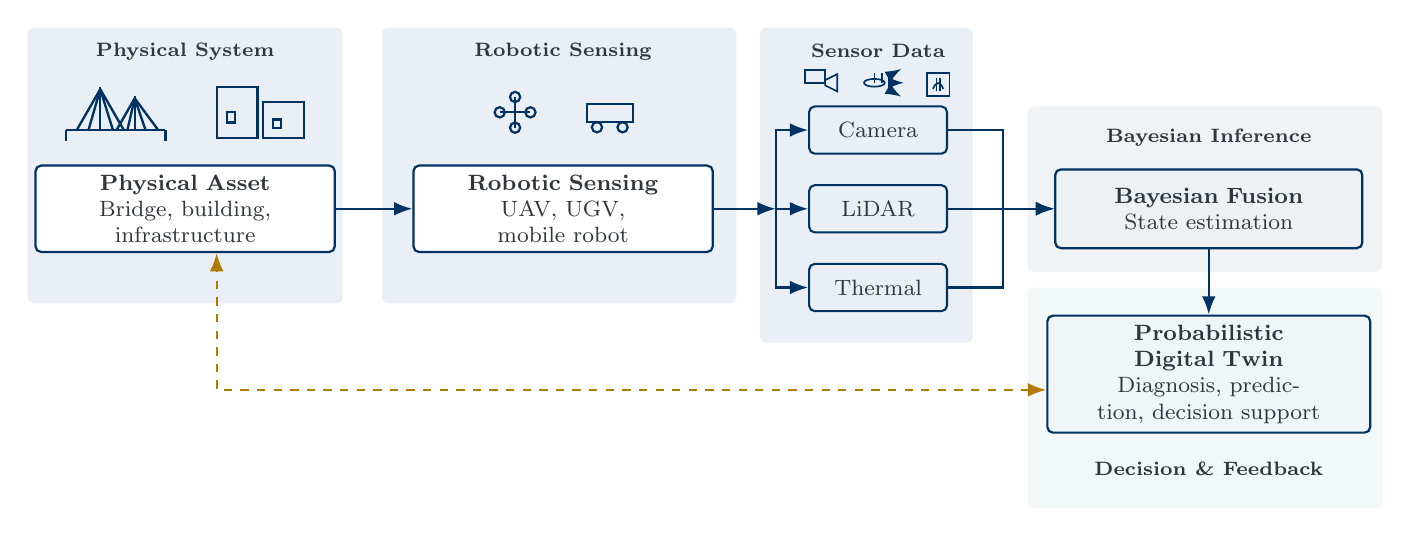
\begin{tikzpicture}[book figure,
    >=Latex,
    font=\footnotesize,
    mainbox/.style={
        draw,
        rounded corners=2pt,
        line width=0.8pt,
        minimum width=3.8cm,
        minimum height=1.05cm,
        text width=3.3cm,
        align=center,
        fill=white
    },
    sensorbox/.style={
        draw,
        rounded corners=2pt,
        line width=0.75pt,
        minimum width=1.75cm,
        minimum height=0.60cm,
        text width=1.35cm,
        align=center,
        fill=BookLight
    },
    fusionbox/.style={
        draw,
        rounded corners=2pt,
        line width=0.8pt,
        minimum width=3.9cm,
        minimum height=1.0cm,
        text width=3.3cm,
        align=center,
        fill=BookBlue!7
    },
    twinbox/.style={
        draw,
        rounded corners=2pt,
        line width=0.8pt,
        minimum width=4.1cm,
        minimum height=1.1cm,
        text width=3.5cm,
        align=center,
        fill=BookTeal!7
    },
    arrow/.style={->, draw=BookBlue, line width=0.8pt},
    feedback/.style={<->, draw=BookGold, dashed, line width=0.8pt},
    stagelabel/.style={font=\scriptsize\bfseries}
]

% ------------------------------------------------
% Background stage bands
% ------------------------------------------------
\begin{scope}[on background layer]
\fill[BookLight,rounded corners=2pt] (-2,2.3) rectangle (2,-1.2);
\fill[BookLight,rounded corners=2pt] (2.5,2.3) rectangle (7,-1.2);
\fill[BookLight,rounded corners=2pt] (7.3,2.3) rectangle (10,-1.7);
\fill[BookBlue!6,rounded corners=2pt] (10.7,1.3) rectangle (15.2,-.8);
\fill[BookTeal!6,rounded corners=2pt] (10.7,-1.0) rectangle (15.2,-3.8);
\end{scope}

% ------------------------------------------------
% Stage labels
% ------------------------------------------------
\node[stagelabel] at (0,2.0) {Physical System};
\node[stagelabel] at (4.8,2.0) {Robotic Sensing};
\node[stagelabel] at (8.8,2.0) {Sensor Data};
\node[stagelabel] at (13.0,0.9) {Bayesian Inference};
\node[stagelabel] at (13.0,-3.3) {Decision \& Feedback};

% ------------------------------------------------
% Boxes
% ------------------------------------------------
\node[mainbox] (asset) at (0,0)
{\textbf{Physical Asset}\\Bridge, building, infrastructure};

\node[mainbox] (robot) at (4.8,0)
{\textbf{Robotic Sensing}\\UAV, UGV, mobile robot};

\node[sensorbox] (cam) at (8.8,1.0) {Camera};
\node[sensorbox] (lidar) at (8.8,0) {LiDAR};
\node[sensorbox] (therm) at (8.8,-1.0) {Thermal};

\node[fusionbox] (fusion) at (13,0)
{\textbf{Bayesian Fusion}\\State estimation};

\node[twinbox] (twin) at (13,-2.1)
{\textbf{Probabilistic Digital Twin}\\Diagnosis, prediction, decision support};

% ------------------------------------------------
% Icons above boxes (larger)
% ------------------------------------------------

% Physical system icon
\begin{scope}[shift={(0.4,0.9)}, line width=0.8pt,scale=1.3]
\draw (0,0) rectangle (0.4,0.5);
\draw (0.45,0) rectangle (0.85,0.35);
\draw (0.1,0.15) rectangle (0.18,0.25);
\draw (0.55,0.1) rectangle (0.63,0.18);
\end{scope}

% Physical system icon: cable-stayed bridge
\begin{scope}[shift={(-1.4,1.0)}, line width=0.85pt, scale=1.15]
    % deck
    \draw (-0.10,0.00) -- (1.00,0.00);
    % pylons
    \draw (0.28,0.00) -- (0.28,0.48);
    \draw (0.66,0.00) -- (0.66,0.38);
    % cables
    \draw (0.28,0.45) -- (0.02,0.00);
    \draw (0.28,0.45) -- (0.15,0.00);
    \draw (0.28,0.45) -- (0.42,0.00);
    \draw (0.28,0.45) -- (0.54,0.00);
    \draw (0.66,0.35) -- (0.46,0.00);
    \draw (0.66,0.35) -- (0.58,0.00);
    \draw (0.66,0.35) -- (0.78,0.00);
    \draw (0.66,0.35) -- (0.92,0.00);
    % supports
    \draw (-0.10,-0.12) -- (-0.10,0.00);
    \draw (1.00,-0.12) -- (1.00,0.00);
\end{scope}

% UAV icon
\begin{scope}[shift={(3.8,0.9)}, line width=0.8pt,scale=1.3]
\draw (0.15,0.25) -- (0.45,0.25);
\draw (0.30,0.10) -- (0.30,0.40);
\draw (0.15,0.25) circle (0.05);
\draw (0.45,0.25) circle (0.05);
\draw (0.30,0.10) circle (0.05);
\draw (0.30,0.40) circle (0.05);
\end{scope}

% UGV icon
\begin{scope}[shift={(5.1,1.1)}, line width=0.8pt,scale=1.3]
\draw (0,0) rectangle (0.45,0.18);
\draw (0.1,-0.05) circle (0.05);
\draw (0.35,-0.05) circle (0.05);
\end{scope}

% ------------------------------------------------
% Small sensor icons inside sensor boxes
% ------------------------------------------------

% Camera icon
\begin{scope}[shift={(-1.2,0.5)}, line width=0.60pt,scale=1.1]
    \draw (8.25,1.00) rectangle (8.48,1.15);
    \draw (8.48,1.03) -- (8.62,1.10) -- (8.62,0.90) -- (8.48,0.97) -- cycle;
\end{scope}

% LiDAR icon
\begin{scope}[shift={(-0.3,1.6)}, line width=0.60pt,scale=1.1]
    \draw (8.23,0.00) ellipse (0.12 and 0.045);
    \draw (8.23,0.11) -- (8.23,0.00);
    \draw (8.32,0.11) -- (8.32,0.00);
    \draw[->] (8.40,0.08) -- (8.54,0.16);
    \draw[->] (8.42,0.00) -- (8.57,0.00);
    \draw[->] (8.40,-0.08) -- (8.54,-0.16);
\end{scope}

% Thermal icon
\begin{scope}[shift={(0.4,2.7)},line width=0.60pt,scale=1.1]
    \draw (8.20,-1.15) rectangle (8.46,-0.89);
    \draw (8.27,-1.07) .. controls (8.31,-0.98) and (8.35,-0.98) .. (8.39,-1.07);
    \draw (8.31,-1.10) -- (8.31,-0.94);
    \draw (8.35,-1.10) -- (8.35,-0.94);
\end{scope}

% ------------------------------------------------
% Flow arrows
% ------------------------------------------------

\draw[arrow] (asset.east) -- (robot.west);

% Branching point moved farther right
\coordinate (j1) at (7.5,0);

\draw[arrow] (robot.east) -- (j1);

\draw[arrow] (j1) |- (cam.west);
\draw[arrow] (j1) -- (lidar.west);
\draw[arrow] (j1) |- (therm.west);

\draw[arrow] (cam.east) -- ++(0.7,0) |- (fusion.west);
\draw[arrow] (lidar.east) -- (fusion.west);
\draw[arrow] (therm.east) -- ++(0.7,0) |- (fusion.west);

\draw[arrow] (fusion.south) -- (twin.north);

\draw[feedback] ([yshift=-2mm]twin.west) -| ([xshift=4mm]asset.south);

\end{tikzpicture}
}
\end{document}
